\chapter{Introduction} \label{chap:intro}
The goal of this thesis is the implementation of a parallel implementation of a pointer analysis. As well as researching to what extent such an implementation presents advantages or disadvantages over other analyses that are not strictly parallel in nature.

\section{Structure of this Thesis}
This thesis is divided into three chapters.
The first chapter \autoref{chap:intro} lays the groundwork for the implementation and goes into detail what ideas were persued in order to develop the implementation. All related current work and it's influences on this work is discussed here, as well as the motivation for the implementation itself. Furthermore the fundamentals of pointer analysis are explained here with code samples and an end to end analysis workflow that aims to illustrate the connection between actual code and its representation in a pointer analysis.

In the second chapter \autoref{chap:main} the software, namely PTAGPU, that was developed as part of this thesis, is described in detail. Design decisions, integrations with other software libraries and correctness are elaborated here.
The experimental benchmark results and how they wre generated are also presented here.

The last chapter \autoref{chap:conclusion} covers possible future work that could further improve the implementation and explore more ideas concerning parallel pointer analyses.
This chapter also discusses the experimental results from \autoref{chap:main}.


\section{Pointer Analysis}
In general a pointer analysis tries to find the values of pointers in a program at runtime, without having to execute the program.
So naturally this problem is undecidable \cite{landi1992undecidability} following a reduction from the halting problem.
As a result, performing a pointer analysis becomes a delicate balancing act between precision and peformance.
Commonly analyses produce over-approximation of the targets each pointer can point towards at runtime while other parts of an analyses might omit or under-approximate certaint parts for the sake of performance and scalability.
As a result, these analyses are strictly speaking unsound or soundy as put forward by \cite{livshits2015defense}:

\begin{quote}
    We introduce the term soundy for
    such analyses. The concept of soundiness
    attempts to capture the balance,
    prevalent in practice, of over-approximated
    handling of most language features, yet deliberately
    under-approximated handling of a feature subset well
    recognized by experts. Soundiness is in
    fact what is meant in many papers that
    claim to describe a sound analysis. A
    soundy analysis aims to be as sound as
    possible without excessively compromising
    precision and/or scalability.
\end{quote}

Pointer analyses build the foundation for a variety of other static analyses, since call-graph generation is directly dependent on pointer analysis in order to resolve indirect or dynamic calls statically.

One common pointer analysis is the inclusion-based Andersen's analysis \cite{andersen1994program}. The details of this type of analysis will be discussed later on, as it is the underlying basis for the proposed algorithm in \autoref{chap:main}. The Andersen algorithm sacrifices precision in favor of performance and achives an upper bound of $O(n^3)$ where n represents the number of pointer variables relevant to the analysis. This is known as the cubic bottleneck of general Andersen analysis \cite{mathiasen2021fine}.
This showcases the tradeoff that all non-theoretical pointer analyses have to make in oder to be applicable to real programs and avoid undecidability. Furthermore Andersen's analysis is a P-complete problem and is therefore not trivially parallelizable.

As a general abstraction, pointer analyses can be seen as complex graph problems where programs are interpreted as graphs with nodes representing variables and edges representing relations between nodes, such as memory allocations and assignments bewteen variables.
This allows us to make use of a large body of previous research concerning graph problems and transform the general analysis into a better defined mathematical problem.

Another analysis closely related to pointer analysis is alias analysis, where two pointers are said to alias if their points-to sets have an intersection. An alias analysis produces a set of relations over all nodes in the analysis graph where nodes can either \textbf{NotAlias}, \textbf{MayAlias} or \textbf{MustAlias}.
For two given nodes, $a$, $b$ and their points-to sets $pts(a)$ and $pts(b)$ the following constraints describe the relations.
$$a\ \textbf{NotAlias}\ b \iff \forall ptd \in pts(a) \colon ptd \notin pts(b)$$
$$a\ \textbf{MayAlias}\ b \iff \exists ptd \in pts(a) \colon ptd \in pts(b)$$
$$a\ \textbf{MustAlias}\ b \iff \forall ptd \in pts(a) \colon ptd \in pts(b)$$
Both pointer analysis, alias analysis, as well as points-to analysis are all terms commonly used interchangeably in literature \cite{hind2001pointer}. From now on pointer analysis will be used in this thesis to refer to this type of static analysis from which an alias relation can be derived based on the pointer information.

A motivating example for pointer analyses is the detection on memory leaks in programs.
This occurs when a memory location is allocated on the heap, for example with a call to malloc in glibc, and is not freed at a later stage in the program.
It is in the interest of the developer to find such faults as to not exhaust the computers memory during execution by repeatedly allocating memory in the heap without freeing previous allocations.
Finding such logical errors can be accomplished via a related static analysis called data-flow analysis, where each possible value at different stages of the program is calculated. Here pointer information is vital, as pointers can represent lateral movement of data trough the control flow of a program, independent of direct assignments and read operations. Ultimately almost all static analyses require some kind of information about pointers to fully determine the state of a program.
Aside from error detection such as memory leaks, optimizations are another aspect of compiler systems, where pointer information is important to achieve better results, see \autoref{lst:dataflow}.
More often than not the pointer information alone does not provide an immediate value to the compiler or analysis tool, instead other procedures build on top of this information to derive valuable information about a program.

\begin{listing}
    \begin{minted}{c}
    #include <stdlib.h>
    void *iter;
    iter = value;

    /* depending on the data at value's memory location 
    the loop might not be necessary */
    
    while(*iter)
    {
        complex_computation(iter);
    }
    \end{minted}
    \caption{Optimizations in a c program}
    \label{lst:dataflow}
\end{listing}

\subsection{Notions of Sensitivity in Pointer Analysis}
As previously established, a complete pointer analysis is undecidable.
For this reason there are various notions of sensitivity when talking about pointer analysis.
These notions represent a compromise between precision, scalability and complexity of the analysis.
Following, some of the more common sensitivity notions will be illustrated to differentiate the more complex analyses from the less complex analyses and explain the impact of these sensitivities on actual performance when analyzing a program.

\subsubsection{Field-sensitivity}
\begin{minted}{c}
int a;
char b;
struct Person {
    char *name;
    int *age;
} p1, p2;
p1.age = &a;
p1.name = &b;
\end{minted}

Field-sensitivity describes how the pointer analysis algorithm handles structures in the program.
Most programming languages that expose memory management to a developer, such as c, c++ and Rust, offer some form of structures to represent an object that internally holds multiple values where these values might be pointers, that reference memory locations.
If an analysis is field-sensitive, each field of each struct is represented in the analysis as an independent node that can point to unique memory locations, as long as the field can be statically determined during the analysis.
If the field of a struct can not be statically determined, for example because of an arithmetic operation that produces multiple possible results for the offset during runtime, it is common for field-sensitive pointer analyses to fallback to a field-insensitive mode for the specific struct, wherein all fields of the struct are merged into a single abstract object.
For the given example, \verb|p1.age| and \verb|p1.name| can point to different memory locations.
Alternatively a field-insensitive analysis does not differentiate between any fields of a given struct at any point of the analysis.
Therefore only two nodes are created to represent the struct, $p1.*$ and $p2.*$.
Another common alternative is field-base-sensitivity, where instead of omitting the individual fields of each struct, the fields of every struct are merged into a single instance of that struct.
As a result the Person structs, p1 and p2, would be represented as a single object with fields name and age, such that \verb|p1.age == p2.age| are represented by the same node in the analysis.

\subsubsection{Array-sensitivity}
Array-sensitivity is conceptually similar to field-sensitivity but often has different effects on the runtime of the analysis.
For a given array $int arr[100]$ an array-sensitivie analysis would model each entry of the array, \newline e.g. arr[0], arr[1], \dots, with a unique node, whereas an insensitive analysis would model the array as a single node.
Generally speaking arrays are often homogeneous data structures that can hold a vast amount of data, compared to structs which are often more compact as they model attributes instead of raw data.
Therefore array-sensitivity if often omitted from whole program analyses, while field-sensitivity is common among pointer analyses.

\subsubsection{Scope of the analysis}
When designing a pointer analysis one has to make a decision about how to handle external code that the program depends on.
Often times a programs transitive dependencies can dwarf the original code by several magnitudes in size \cite{toman2017taming}.
Even a basic Hello World program in Java transitively depends on 3000 classes \cite{kulkarni2016accelerating} from the Java standard library.
For this reason most analyses either ignore external library code during analysis, or stub the most relevant library calls during analysis, such as \verb|malloc| or \verb|free|.
This tradeoff is well worth it, as most interesting properties in pointer analysis do not originate in extenal libraries, but the actual program code that is written by the developer.
This does however not solve the problem of standard library code mutating the program state either via callbacks or mutation of values behind pointer arguments. Here, simply ignoring the external code during analysis would greatly decrease the accuracy of the analysis.
For this reason, a lot of research is being done to develop methods that alleviate some of the problems that arise from analyzing external dependencies of a given program. Caching incremental results during analysis seems to be one of the most promising methods thus far \cite{mcpeak2013scalable}, where instead of solving the pointer analysis problem from the top-down, the analysis begins at the bottom and builds summaries for functions incrementally until a result over the entire program is achieved. Hybrid approaches combining top-down and bottom-up analysis represent state of the art analysis methods in use by production static analysis tools, such as Coverity \cite{mcpeak2013scalable}.

\subsubsection{Interprocedural analysis}
Another aspect that greatly influences the precision of analyses is whether they are interprocedural or intraprocedural.
An intraprocedural analysis only analyzes each function in an isolated context and disregards any influences on other functions or global state.
Interestingly most compilers rely mostly on intraprocedural analysis for bug detection as it can be performed in parallel for each function independently and is in general much faster than interprocedural analysis.
The following example \ref{lst:intraprocedural} illustrates the shortcomings of only performing intraprocedural analysis. Essentially parameter passing especially of pointers is not taken into account properly for the calculation of points-to sets.
An interprocedural analysis overcomes these limitations by connecting parameters of functions and the arguments at the respective callsites as well as the resulting return values in the graph structure that is used to solve the pointer analysis.
Fundamentally an interprocedural analysis is related to another notion of sensitivity, context sensitivity, since every context sensitive analysis has to be interprocedural in order to capture the context of each function call \cite{lin2015alias}.

\begin{listing}
    \begin{minted}{c}
        int *manupulatePointer(int *ptr);
        int main() {
            int *a, *b;
            b = manupulatePointer(a);
            /* intraprocedural analysis is unable 
            to determine the state of a or b */
        }
    \end{minted}
    \caption{Limitations of intraprocedural analysis}
    \label{lst:intraprocedural}
\end{listing}


\subsubsection{Flow-sensitivity}
When one performs a flow-sensitive pointer analysis, this means that the analysis takes into account the control flow of the program when calculating point-to information.
As can be seen in \ref{lst:flowsens}, a flow-sensitive analysis is in general more precise than a flow-insensitive analysis. Meanwhile running a flow-sensitive analyis is also exponentially more expensive to compute as every step in a programs control flow carries its own state concerning points-to relations - especially when the control flow is complicated by complex conditional statements or recursive execution.
Although this problem can be slightly alleviated, by only condering program statements that manipulate pointers.
Using a flow-sensitive pointer analysis also generates must-alias relations, compared to the comparatively imprecise may-alias relations from a flow-insensitive pointer analysis.
Generating definitive information that two variables will unconditionally alias during runtime is very valuable when considering refactoring optimizations by a compiler.
While a sound may-alias analysis requires that no possible alias relations are missed, a sound must-alias analysis requires analogously that no spurious alias relations are reported. Both are respectively over- and under-approximations of the true points-to results.

\begin{listing}
    \begin{minted}{c}
        int *manupulatePointer(int *ptr);
        int main() {
            int a, b, *x; // x -> {}
            if (something())
                x = &a; // x -> {a}
            else
                x = &b; // x -> {a,b} ?
            manupulatePointer(x);
            /* a flow insensitive analysis computes 
            a points-to set {a,b} for x while in actuality 
            x = &b and x = &a are mutually exclusive statements
            during execution */
        }
    \end{minted}
    \caption{Flow-sensitivity by example}
    \label{lst:flowsens}
\end{listing}

\subsubsection{Context-sensitivity}
As previouly eluded to, context-sensitivity is directly related to interprocedural analyses, since it governs how call sites and called functions are interpreted during the analysis.
More specifically a centext-sensitive analysis tries to qualify variables both on the heap and stack with contextual information such that different contexts can be established, where for example points-to information for a variable differs, thus improving the precision of the analysis.
To achieve this context-sensitivity can be modeled by using call-sites and objects to differentiate qualify the context for variables \cite{smaragdakis2015pointer}. Depending on the programming language at hand, these methods can yield different precision. It has been established that object oriented languages like Java greatly benefit from object-sensitivity over call-site-sensitivity, while more procedural languages like C benefit from call-site-sensitivity.
While a context-sensitive analysis would in theory provide more precision and therefore decrease the average size of points-to sets, in practice most context-sensitive pointer analyses, when applied to sizeable codebases, quickly grow out of control as the analysis explodes in terms of running time and space requirements \cite{smaragdakis2014introspective}. In contrast, context-insensitive analyses anecdotally scale better than context-sensitive analyses.

\cite{smaragdakis2015pointer} for flow and context sens

\begin{listing}
    \begin{minted}{c}
        int *manupulatePointer(int *ptr);
        int main() {
            int a, b, *x;
            x = &a;
            manupulatePointer(x);
            x = &b;
            manupulatePointer(x);
            /* a context-sensitive analysis evaluates both
            calls to manupulatePointer as unique function calls
            since the context differs between both calls */
        }
    \end{minted}
    \caption{Context-sensitivity by example}
    \label{lst:contextsens}
\end{listing}

heap abstractions \cite{kanvar2016heap}

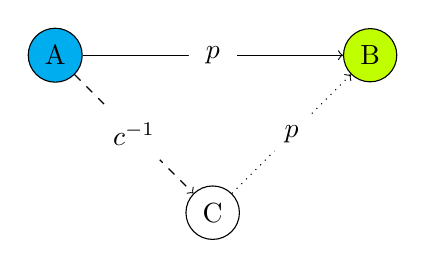
\begin{tikzpicture}
    \node[shape=circle,draw=black,fill=cyan] (A) at (0,0) {A};
    \node[shape=circle,draw=black,fill=lime] (B) at (4,0) {B};
    \node[shape=circle,draw=black] (C) at (2,-2) {C};
    
    \path [->] (A) edge[] node[fill=white,circle] {$p$} (B);
    \path [->] (A) edge[dashed] node[fill=white,circle] {$c^{-1}$} (C);
    \path [->] (C) edge[dotted] node[fill=white,circle] {$p$} (B);
\end{tikzpicture}

\begin{tikzpicture}
    \begin{scope}[every node/.style={circle,thick,draw}]
        \node (A) at (0,0) {A};
        \node (B) at (0,3) {B};
        \node (C) at (2.5,4) {C};
        \node (D) at (2.5,1) {D};
        \node (E) at (2.5,-3) {E};
        \node (F) at (5,3) {F} ;
    \end{scope}
    
    \begin{scope}[>={Stealth[black]},
        every node/.style={fill=white,circle},
        every edge/.style={draw=red,very thick}]
        \path [->] (A) edge node {$5$} (B);
        \path [->] (B) edge node {$3$} (C);
        \path [->] (A) edge node {$4$} (D);
        \path [->] (D) edge node {$3$} (C);
        \path [->] (A) edge node {$3$} (E);
        \path [->] (D) edge node {$3$} (E);
        \path [->] (D) edge node {$3$} (F);
        \path [->] (C) edge node {$5$} (F);
        \path [->] (E) edge node {$8$} (F);
        \path [->] (B) edge[bend right=60] node {$1$} (E);
    \end{scope}
\end{tikzpicture}

field - flow - context - array sensitivity; structure sensitivity: \cite{balatsouras2016structure}
\subsection{Andersen's Analysis}
Andersen's analysis is an inclusion based interprocedural pointer analysis algorithm first proposed by \cite{andersen1994program} in 1994. It is a field-sensitive, context-insensitive and flow-insensitive analysis. 
The algorithm was one of the first constraint based algorithms introduced for pointer analysis. Since it is lacking constext- and flow-sensitivity, it is often used as a base algorithm which produced broad over estimations of the points-to data and is later refined by more precise algorithms which improve the quality of the data and remove false positives from the points-to information generated by Andersen's algorithm.
%Boyond the originally proposed Andersen Algorithm there have been multiple adaptations of the algorithm which
The underlying idea is that the Algorithm operates on a given program by converting statements from the program into mathematical constraints.
These constraints can be classified into a few types which can be seen in \autoref{tab:ander}.
It is worth noting that in literatur the field-sensitivity aspect is often omitted from the definition of the Andersen analysis although it was included in the original specification.
As mentioned in \autoref{chap:intro} the complexity of Andersen's analysis grows exponentially with regards to the number of pointer variables in a program. The reason for this exponential growth, among other aspects, is the field-sensitivity. Depending on the structure of the code under analysis, field-sensitivity might play the most influential part in the analysis' complexity. This will be further expanded upon in \autoref{chap:main}. Ultimaltely this is the reason for specifically including field-sensitivity when discussing Andersen's analysis in this thesis.
\begin{table}
    \begin{center}
        \caption{Constraints of an inclusion-based pointer analysis.}
        \label{tab:ander}
        \begin{tabular}{l|c|l}
            \hline                                                                                                         \\
            \textbf{Statement} & \textbf{Description}                        & \textbf{Constraint}                         \\
            \hline                                                                                                         \\
            $x = \&a$          & The address of a is assigned to variable x. & $\{a\} \subseteq pts(x)$                    \\
            $x = y$            & Variable y is assigned to x.                & $pts(y) \subseteq pts(x)$                   \\
            $x = *y$           & Load value of y and assign to x.            & $\forall p \in y \colon p \subseteq pts(x)$ \\
            $*x = y$           & Store y into value of x.                    & $\forall p \in x \colon y \subseteq pts(p)$ \\
            $x = y.f$          & Field f of variable y is assigned to x      & $pts(y.f) \subseteq pts(x)$                 \\
        \end{tabular}
    \end{center}
\end{table}

\subsection{Steensgard's Analysis}
Steensgard's analysis was introduced in 1996 by \cite{steensgaard1996points}. It was inspired by Andersen's analysis and as such is also an interprocedural pointer analysis.
The key proposition of Steensgard's work was to improve the runtime of Andersen's algorithm by using equalities instead of subsets for the constraints that are used as inputs for the algorithm, an overview for the constraints can be seen in \autoref{tab:steens} - the rules are nearly identical to the constraints for the Andersen algorithm.
The change from subsets to equalities leads to an almost linear algorithm by utilizing union/find datastructures for efficient computation of a fixpoint solution for a given set of pointers.
The tradeoff for this faster algorithm is precision, since Steensgard's algorithm quickly looses precicion compared to Andersen's algorithm by loosing the small differences between points-to sets of individual varialbes by equating them. An example for this precision loss can be seen in \autoref{lst:steensvander}.

\begin{listing}
    \begin{minted}{c}
        int main() {
            int a, b, *x, *y;
            x = &a; // pts(x) = {a}
            y = &b; // pts(y) = {b}
            y = x; // pts(y) = pts(x) = {a,b}
            /* by equating the points-to sets of x and y
            the fact that x never points to b is lost
            this leads to an obvious loss of precision */
        }
    \end{minted}
    \caption{Steensgard easily looses precision.}
    \label{lst:steensvander}
\end{listing}

\begin{table}
    \begin{center}
        \caption{Constraints of an equality-based pointer analysis.}
        \label{tab:steens}
        \begin{tabular}{l|c|l}
            \hline                                                                                                 \\
            \textbf{Statement} & \textbf{Description}                        & \textbf{Constraint}                 \\
            \hline                                                                                                 \\
            $x = \&a$          & The address of a is assigned to variable x. & $\{a\} \subseteq pts(x)$            \\
            $x = y$            & Variable y is assigned to x.                & $pts(y) = pts(x)$                   \\
            $x = *y$           & Load value of y and assign to x.            & $\forall p \in y \colon p = pts(x)$ \\
            $*x = y$           & Store y into value of x.                    & $\forall p \in x \colon y = pts(p)$ \\
            $x = y.f$          & Field f of variable y is assigned to x      & $pts(y.f) = pts(x)$                 \\
        \end{tabular}
    \end{center}
\end{table}

inclusion based pta idea, timeframe
\subsection{Wave Propagation}
explain optimizations in modern sequential pta implementations: diffpts, worklists, consed hashes, \cite{waveprop}
\subsection{LLVM - Generating Data for Analysis}
By now the fundamentals of pointer analysis have been introduced, which unilaterally can be modeled as a graph problem.
The missing part of the Introduction is where the underlying data for such a pointer analysis algorithm comes from or how it is derived from a given program that has to be analyzed.
Initially pointer analyses were solely implemented in compilers to detect errors and find possible optimizations during compilation. As compilers already employ an internal representation for the programs to be compiled, the data generation was not problematic.
As the scope of pointer analyses expands from intraprocedural analysis part of a compiler towards standalone interprocedural whole program analyses it is clear, that a new representation for programs is needed, on which analyses can run - independent of compilations.

During initial review of literature for pointer analysis multiple methods for data generation were surveyed. Notably parsing was among the most common data extraction methods for programs. Another method was to extract an intermediate representation, called LLVM-IR, of the code during compilation of a program by means of using the low level virtual machine, LLVM. Using LLVM has some distinct advantages compared to parsing the source files of a program directly.
For one, LLVM provides multiple compiler front-ends for various compiled programming languages, including C/C++ and Objective-C through the Clang compiler, which allows one to compile multiple languages without having to adapt the parser, as can be seen in \autoref{fig:llvm}.
Especially when working with older non-strictly standardized versions of the C language, utilizing all available tricks of an established compiler proves to be more resourceful compared to reinventing the wheel with new parsing tools.
Secondly one can easily verify the correctness of the extracted data for a program by simply executing the compiled intermediate representation since no matter the programming language, as part of the llvm toolchain the program always gets compiled into the intermediate representation before being assembled and linked. The LLVM project provides specific tools for executing programs in LLVM-IR format using a just-in-time compiler \footnote{https://releases.llvm.org/9.0.1/docs/CommandGuide/lli.html}. Beyond the binary intermediate representation, also called bitcode, there exists a human-readable format. Both binary and text versions can be converted between with the llvm tools \verb|llvm-as| and \verb|llvm-dis|, see \autoref{lst:llvmir} for a basic hello world program in human-readable LLVM-IR.

\begin{figure}
    \centering
    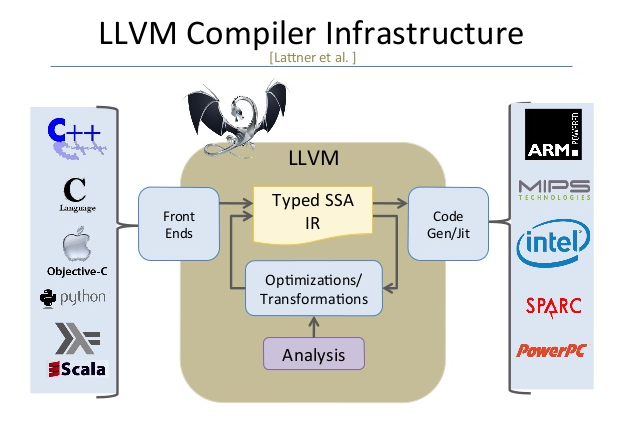
\includegraphics[width=1.\textwidth]{img/llvm.png}
    \caption{Illustration of the LLVM toolchain from Lattner et al.}
    \label{fig:llvm}
\end{figure}

\begin{listing}
    \begin{minted}{c}
#include <stdio.h>
int main()
{
    printf("Hello World!\n");
    return 0;
}
// gets compiled into...
    \end{minted}
    \begin{minted}{llvm}
@.str = private unnamed_addr constant [14 x i8] c"Hello World!\0A\00", align 1
; Function Attrs: noinline nounwind optnone uwtable
define dso_local i32 @main() #0 {
    %1 = alloca i32, align 4
    store i32 0, i32* %1, align 4
    %2 = call i32 (i8*, ...) @printf(i8* getelementptr inbounds 
        ([14 x i8], [14 x i8]* @.str, i64 0, i64 0))
    ret i32 0
}
declare dso_local i32 @printf(i8*, ...) #1
    \end{minted}
    \caption{A basic hello world program in human-readable LLVM-IR.}
    \label{lst:llvmir}
\end{listing}


go through instrs, and how they are relevant to pta, explain constraints \cite{lin2015alias}
\section{Related Work}
\subsection{Context Free Languages}
first general idea: \cite{reps1998program} first idea of gemm for cflpq \cite{azimov2018context} kronecker product idea \cite{orachev2020context} evaluation \cite{mishin2019evaluation} spbla library \cite{orachev2021spbla}, current draft [Taming Transitive Redundancy for Context-Free Language Reachability] fron SVF, parallel pta via cfl \cite{su2014parallel}
\subsection{Sequential Analyses}
\subsubsection{SVF}
svf idea, built on top of llvm, \cite{sui2016svf}, briefly explain all subcomponents i.e. memleak detection: \cite{sui2014detecting} demand driven VF: \cite{sui2018value} new alternative, faster, better results than svf \cite{shi2018pinpoint}
\subsection{GPU Accelerated Analyses}
\subsubsection{Graspan}
original idea \cite{zheng2008demand} big data approach on cpu \cite{wang2017graspan} and gpu \cite{zuo2021systemizing} alternative impl \cite{gu2020towards} based on \cite{mendez2012gpu} and \cite{mendez2010parallel}
\section{Motivation}
general alias analysis is undecidable
\subsection{Static Analysis in Software Development}
finding bugs is becoming harder

inter procedural analysis scalability; create a single machine implementation that used parallel hardware and integrates into SVF

This is a citation \cite{juliani2018unity}!

\begin{figure}
    \centering
    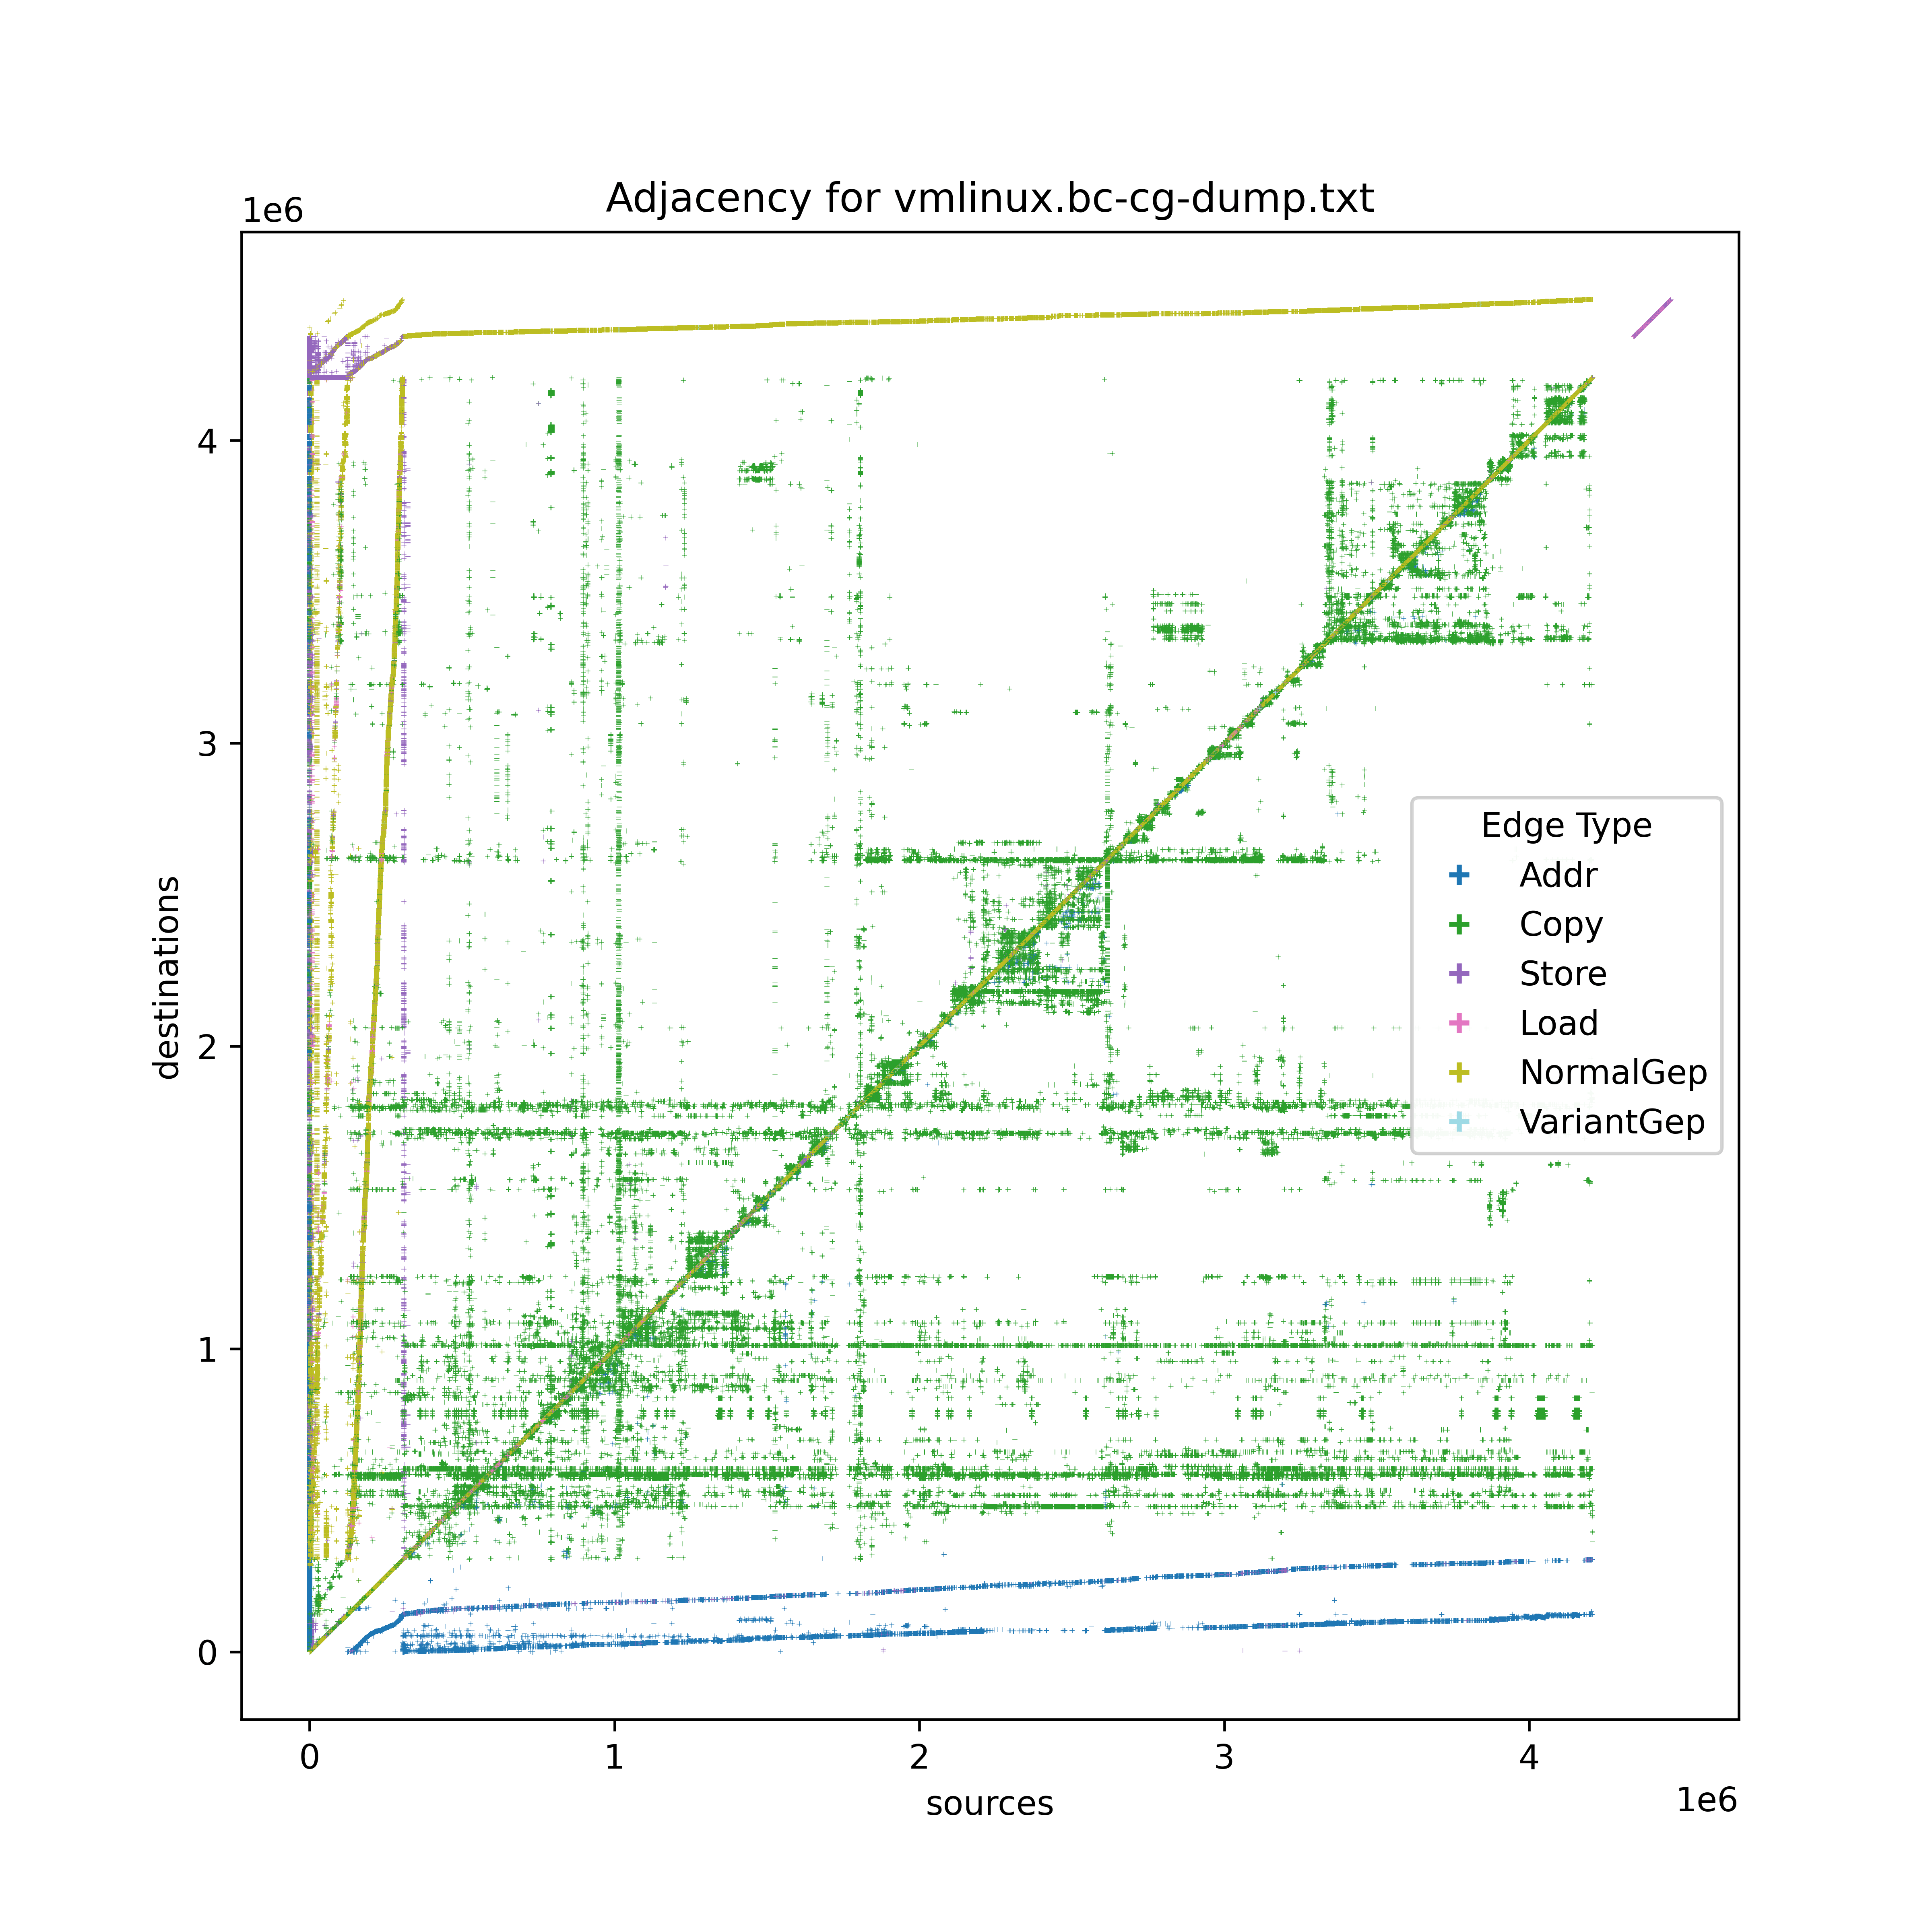
\includegraphics[width=1.\textwidth]{img/linux-consg-min.png}
    \caption{Adjacency Plot for the Constraint Graph of the Linux Kernel}
    \label{fig:linux-consg}
\end{figure}


\begin{table}
    \begin{center}
        \caption{More rows.}
        \label{tab:table1}
        \begin{tabular}{l|S|r}
            \textbf{Value 1} & \textbf{Value 2} & \textbf{Value 3} \\
            $\alpha$         & $\beta$          & $\gamma$         \\
            \hline
            1                & 1110.1           & a                \\
            2                & 10.1             & b                \\
            3                & 23.113231        & c                \\
            4                & 25.113231        & d                \\ % <-- added row here
        \end{tabular}
    \end{center}
\end{table}
